\chapter{Antecedentes Conceptuales}\label{cap2}

\section{Teoría de Grafos}
\label{sec:teoria_grafos}
La teoría de grafos es un rama que estudia las propiedades de los grafos. Concibe formalismos para representarlos de manera matemática, como también de forma gráfica. Un grafo $G=(V,E,\psi)$ está definido por un conjunto de vértices o nodos $V$, un conjunto de aristas o arcos $E$ y una función $\psi$ que asocia cada arista en $E$ con un par no ordenado de vértices en $V$ \cite{bondy1976graph}\cite{dubinsky1984mathematical}.

Los grafos pueden ser representados gráficamente a partir del dibujado sobre un plano de sus vértices como puntos y sus aristas como líneas que conectan tales puntos. 

\subsection{Estilos de Dibujado de Grafos}
\label{sec:estilos_de_dibujado}
 Para poder dibujar un grafo se debe, mínimamente, posicionar cada vértice sobre un punto $(x,y)$ sobre el plano, y luego unirlos mediante líneas según correspondan sus aristas. Dependiendo del estilo que se utilice los aristas pueden dibujarse como líneas rectas, curvas o por cadenas poligonales (líneas articuladas) \cite{nishizeki2004planar}.
 
\subsubsection{Dibujado Planar}
Un dibujado planar de un grafo es aquel en la que no hay intersección entre ningún par de aristas. Es posible dibujar un grafo de manera planar o no planar, pero no todos los grafos tienen un dibujado planar. Un grafo que admite al menos un dibujado planar es llamado grafo planar.

\begin{figure*}[h]
	\centering
	\subfigure[Grafo dibujado de manera planar]{
		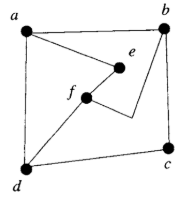
\includegraphics[width=0.33\textwidth]{imagenes/grafo_planar_1.png}
		\label{subfig:ejemplo_dibujado_planar}
	}
	\subfigure[El mismo grafo dibujado de manera no planar]{
		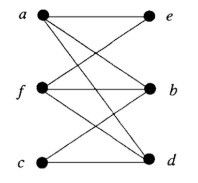
\includegraphics[width=0.33\textwidth]{imagenes/grafo_no_planar_1.png}
		\label{subfig:ejemplo_dibujado_no_planar}
	}
	\caption{Ejemplo de grafo planar. Dibujado de manera planar y no planar \cite{nishizeki2004planar}.}
	\label{fig:ejemplo_dibujado_planar}
\end{figure*}

\subsubsection{Dibujado Diagrama de Arcos}
\label{sec:dibujado_diagrama_de_arcos}

Un Diagrama de Arcos \cite{Wat02} es un estilo con el  que se dibuja un grafo, en el que los vértices del grafo se ubican sobre  una línea en el plano  Euclídeo y los arcos se dibujan como  semicírculos sobre alguno de los dos  semiplanos delimitados por la línea o bien pueden ser segmentos de la línea, siempre que conecten vértices que son consecutivos en la recta.
En la Figura \ref{fig:arcdiagram_ejemplo} se muestra un ejemplo con 6 nodos.

\begin{figure}[h]
	\centering
	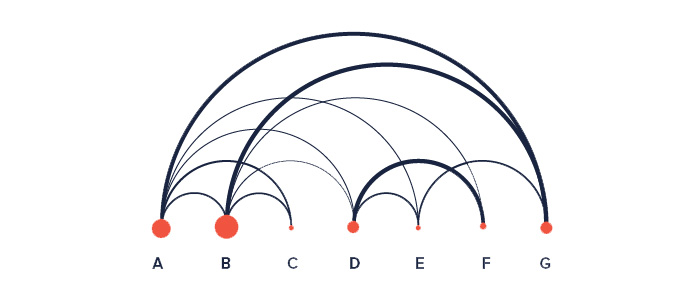
\includegraphics[width=12cm]{imagenes/diagrama-de-arco.jpg}
	\caption{Ejemplo de un diagrama de arcos.}
	\label{fig:arcdiagram_ejemplo}
\end{figure}

%imagen de grafo arc diagram

\subsection{Propiedades de Dibujado de Grafos}
\label{sec:propiedades_dibujado_grafos}
Los grafos pueden dibujarse de infinitas formas, pero al momento de dibujar un grafo para un uso específico se consideran una variedad de propiedades que brindan medidas para fortalecer ciertas características que quieran destacarse o mejorarse de un dibujo para así hacerla mas intuitiva según su dominio.\\

\begin{property}[Área]
	Es el área que ocupa el plano donde se dibuja el grafo. Si el área es de gran tamaño, produce que tengamos que visualizarlo mediante muchas páginas o desplazarnos sobre el plano. En cambio, si disminuimos la resolución se vuelve mas dificultoso de leer. En este sentido, se busca una relación de aspecto favorable entre el tamaño y la resolución.
\end{property}

\begin{property}[Cruces de Arcos]
	Los cruces o intersecciones de arcos abren a posibles confusiones de lectura, por lo que en cualquier dibujado siempre se busca disminuir lo mas posibles la cantidad de cruces.
\end{property}

\subsection{Aplicaciones de grafos}
Pueden utilizarse los grafos para diversas aplicaciones. Una de principal interés es la visualización de modelos conceptuales, permitiendo representarlos ante una notación particular de cada tipo de modelado.

%imagenes de modelos conceptuales (uml, er, orm)

\section{Problemas NP}
\label{sec:problemas_np}
Los problemas NP son aquellos que se encuentran categorizados en la clase de complejidad temporal NP (\emph{nondeterministic polynomial  time}). La clase NP abarca un conjunto de problemas de decisión los cuales pueden ser resueltos en un tiempo polinomial por una Máquina de Turing No Determinística, a partir de ahora MTND \cite{arora2009computational}.

Formalmente en términos de $\text{NTIME}$ se define como:

$$\text{NP} = \bigcup_{k \in  \mathbb{N}}^{}{\text{NTIME}(n^k)}$$

donde $\text{NTIME}(n^k)$ es el conjunto de problemas que pueden resolverse por una MTND en tiempo $O(n^k)$.

Entre estos problemas se considera de interes el problema de Crossing Number.

\subsection{Crossing Number}
\label{sec:crossing_number}
Una de las propiedades fundamentales de dibujado de grafos \ref{sec:propiedades_dibujado_grafos} es el número de cruces de arcos, \emph{crossing number} a partir de ahora, o $v(G)$ de un grafo $G=(V,E)$. Esta es, el menor número entero $K$ tal que $G$ puede ser dibujado en el plano, donde no haya mas de $K$ intersecciones entre los arcos graficados del conjunto $E$.

En general, el problema de decisión de \emph{crossing number} se define como ``Dado un grafo $G$ y un número entero $K$, ¿es $v(G) \leq K$?"

Este problema es considerado dentro de la clase de complejidad NP \cite{garey1983crossing}.

\section{Algoritmos de Layout de Grafos}
Los algoritmos de layout de grafos responden a una clase particular de problemas de optimización combinatorios, cuyo objetivo es encontrar un layout lineal de un grafo de entrada de manera que una determinada función sea optimizada. Un layout lineal es un etiquetado de los nodos de un grafo con un número entero distintivo \cite{diaz2002survey}, como se muestra en la figura \ref{fig:ejemplo_grafo_linear}.

\begin{figure*}[h]
	\centering
	\subfigure[Grafo etiquetado con un layout lineal.]{
		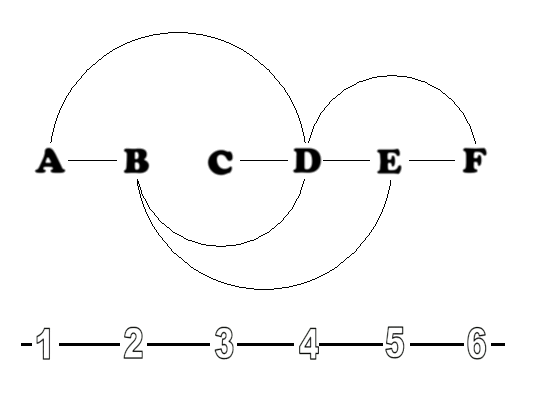
\includegraphics[width=0.39\textwidth]{imagenes/grafo_linear_2.png}
		\label{subfig:ejemplo_grafo_linear_original}
	}
	\subfigure[El mismo grafo etiquetado con otro layout lineal.]{
		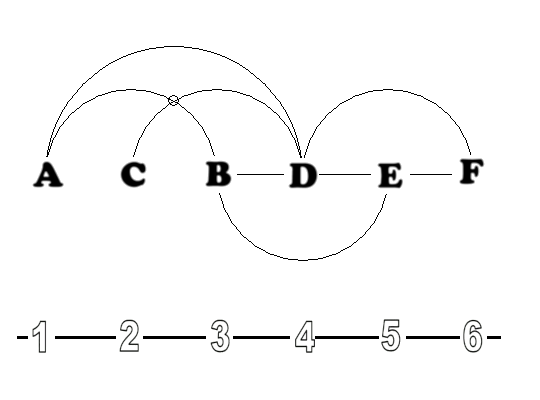
\includegraphics[width=0.39\textwidth]{imagenes/grafo_linear_1.png}
		\label{subfig:ejemplo_grafo_linear_otro_orden}
	}
	\caption{Ejemplo de layout lineal con nodos etiquetados del 1 al 6.}
	\label{fig:ejemplo_grafo_linear}
\end{figure*}

Un gran número de problemas relevantes de diferentes dominios pueden ser formulados como un problema de layout de grafos. Esto incluye, optimización de redes para arquitecturas de computadoras paralelas, diseño de circuitos VLSI (Very Large-Scale Integration), gestión de información, análisis numérico, biología computacional, teoría de grafos \ref{sec:teoria_grafos}, planificación y arqueología. Los problemas mas interesantes de layout de grafos son problemas NP-Hard y sus equivalentes problemas de decisión NP-Completos que son mencionados en la sección \ref{sec:problemas_np}, pero, para la mayoría de sus aplicaciones, es suficiente con soluciones factibles que consigan aproximadamente un costo óptimo. Como consecuencia, algoritmos aproximados y heurísticas efectivas son bienvenidas en la práctica.

% Graph layout problems are a particular
% class of combinatorial optimization problems
% whose goal is to find a linear layout
% of an input graph in such a way that a
% certain objective function is optimized. A
% linear layout is a labelling of the vertices
% of a graph with distinct integers. A large
% number of relevant problems in different
% domains can be formulated as graph layout
% problems. These include optimization
% of networks for parallel computer architectures,
% VLSI circuit design, information
% retrieval, numerical analysis, computational
% biology, graph theory, scheduling
% and archaeology. Most interesting graph
% layout problems are NP-hard and their
% decisional versions NP-complete, but, for
% most of their applications, feasible solutions
% with an almost optimal cost are sufficient.
% As a consequence, approximation
% algorithms and effective heuristics are
% welcome in practice.

\section{Algoritmos Evolutivos}
En la naturaleza, la evolución es mayormente determinada por la selección natural de diferentes individuos compitiendo en un ambiente. Aquellos individuos que son mejores son más aptos para sobrevivir, y propagar su material genético. La codificación para la información genética (genoma) esta dada en una forma que admita la reproducción asexual, lo que resulta en una descendencia que es genéticamente idéntica a sus padres.

La reproducción sexual permite el intercambio y re-ordenamiento de algunos cromosomas, produciendo una descendencia que contiene una combinación de la información genética de cada padre. Esta es la operación de \emph{recombinación}, que normalmente es llamada \emph{crossover} (o cruzamiento) debido a la manera en que los cromosomas se cruzan durante el intercambio. La diversidad en la población es lograda mediante la operación de \emph{mutación} \cite{grosan2011intelligent}.

% In nature, evolution is mostly determined by natural selection of different individuals
% competing for resources in the environment. Those individuals that are better
% are more likely to survive and propagate their genetic material. The encoding
% for genetic information (genome) is done in a way that admits asexual reproduction,
% which results in offspring that are genetically identical to the parent.
% Sexual reproduction allows some exchange and re-ordering of chromosomes, producing
% offspring that contain a combination of information from each parent. This
% is the recombination operation, which is often referred to as crossover because of
% the way strands of chromosomes cross over during the exchange. The diversity in
% the population is achieved by mutation operation.

Este concepto se agrupa usualmente sobre el término \emph{Computación Evolutiva} o \emph{Algoritmos Evolutivos} \cite{back1997handbook}\cite{back1996evolutionary}, y sobre estos encontramos el dominio de los \emph{Algoritmos Genéticos} \cite{holland1992adaptation}\cite{goldberg1989genetic}, el cuál se describe en la sección \ref{sec:algoritmos_geneticos}, y otros como la \emph{Programación Evolutiva}\cite{fogel1966artificial}, la \emph{Programación Genética} \cite{koza1992genetic}\cite{michalewicz1996genetic} y las \emph{Estrategias de Evolución} \cite{vent1975rechenberg}\cite{schwefel1977evolutionsstrategien}. Todos ellos comparten la misma base conceptual de simular la evolución de estructuras de individuos mediante un proceso de selección, recombinación y mutación, y de esta manera producir mejores soluciones. Los procesos dependen del desempeño percibido de las estructuras de individuos definidas por el problema particular. Este es un proceso iterativo como el que se puede ver en la figura \ref{fig:esquema_evolutivo}.
\begin{figure}[h]
	\centering
	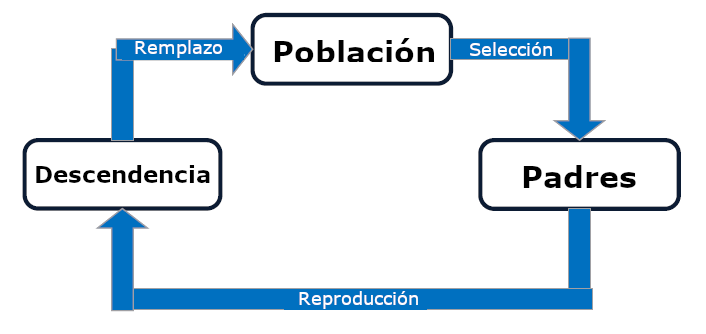
\includegraphics[width=8cm]{imagenes/esquema_evolutivo.png}
	\caption{Esquema de algoritmo evolutivo \cite{grosan2011intelligent}.}
	\label{fig:esquema_evolutivo}
\end{figure}

% Usually grouped under the term evolutionary computation or evolutionary algorithms
% [1][4], we find the domains of genetic algorithms [9], evolution strategies
% [26][27], evolutionary programming [28] and genetic programming [29].
% They all share a common conceptual base of simulating the evolution of individual
% structures via processes of selection, recombination and mutation reproduction and
% thereby producing better solutions. The processes depend on the perceived performance
% of the individual structures as defined by the problem. The procedure is
% then iterated as illustrated in Figure 14.1.

\section{Algoritmos Genéticos}
\label{sec:algoritmos_geneticos}
Los algoritmos genéticos son algoritmos de búsqueda, que al igual que los evolutivos, están basados en la selección natural, pero en este caso también se utilizan comportamientos de la genética en la naturaleza. Estos combinan la supervivencia del mas apto entre estructuras basadas en strings (cadenas de caracteres) con un intercambio de información estructurada pero aleatorizada para, de esta manera, formar un algoritmo de búsqueda con un estilo similar al de la búsqueda humana. En cada generación, un nuevo grupo de criaturas artificiales (strings) es creado creada y representada mediante bits procedentes de sus antecesores y nuevas partes. A pesar de ser aleatorios, los algoritmos genéticos no son simples búsquedas aleatorias. Estos aprovechan la información histórica para encontrar nuevos puntos de búsqueda de los que se espera una mejora con respecto a los anteriores \cite{goldberg1989genetic}.

Los algoritmos genéticos son probablemente el tipo de algoritmos evolutivos mas utilizados y simple de implementar para cualquier tipo de problema de optimización. Estos presentan diferentes maneras de diseñar la representación de los individuos, los mecanismos de selección y las operaciones de variación (recombinación y mutación) \cite{grosan2011intelligent}.

\subsection{Representación de Individuos}
La representación de los individuos es uno de los pasos mas importantes en el diseño de un algoritmo genético. La representación debe ser adecuada para el problema que se quiere resolver y debe consumir la menor cantidad de recursos posibles. Para un problema pueden haber múltiples posibles representaciones; por esto, tenemos que determinar cual es la mas adecuada para satisfacer las necesidades y requerimientos del problema \cite{grosan2011intelligent}.

Existen tipos estándar de representación de individuos, los cuales permiten utilizar la misma forma para diferentes problemas pero cambiando la interpretación que se les da. Algunas de las mas importantes son las siguientes:
\begin{itemize}
    \item Representación Binaria.
    \item Representación Entera.
    \item Representación Real o Flotante.
    \item Representación basada en Orden o Permutación.
\end{itemize}

\subsection{Inicialización de la Población}
El próximo paso en el desarrollo de un algoritmo genético es la inicialización de la población. Esto significa dar un semilla para generar aleatoriamente un número dado de individuos teniendo en cuenta la codificación/representación elegida. Mientras se realiza la generación, existen posibilidades que algunos individuos puedan tener múltiples copias de si mismos \cite{grosan2011intelligent}.

Para cada representación particular, existen diferentes técnicas para inicializar la población. Por ejemplo:

\begin{itemize}
    \item Para una representación binaria: un individuo esta representado por un string con valores de $\{0, 1\}$, por lo tanto los genes deberán inicializarse con valores $0$ o $1$ de manera equiprobable.
    \item Para una representación basada en orden: el individuo esta dado por una permutación de tamaño $n$. Cada gen $i$ deberá ser inicializado con valores entre $\{1, ..., n\}$ donde el valor no debe ocurrir en las posiciones previamente inicializadas.
\end{itemize}

\subsection{Mecanismos de Selección}
El proceso de selección en un algoritmo genético ocurre cuando los potenciales candidatos que para ser usados en el crossover son seleccionados. De manera estándar, los individuos mas aptos, con mayor \emph{fitness} a partir de ahora, son aquellos con mayor probabilidad de ser seleccionados \cite{grosan2011intelligent}.

Algunos de los mecanismo de selección mas utilizados son:

\begin{itemize}
    \item Selección por Torneo.
    \item Selección proporcional al fitness.
    \item Selección por Ruleta.
    \item Selección basada en Rango.
\end{itemize}

\subsection{Operaciones de Variación}
Las operaciones de variación principales son recombinación o \emph{crossover} y mutación. Cada una de ellas tienen formas especificas según las diferentes representaciones de individuos \cite{grosan2011intelligent}.

\subsubsection{Crossover o Recombinación}
El rol de la operación de \emph{crossover} es el de producir nuevos individuos combinando la información contenida en dos o mas padres. Esto se logra combinando los genes de los padres. Dependiendo en que representación estén dados tales genes, diferentes métodos serán utilizados y para estos también diferentes maneras de implementarlos \cite{grosan2011intelligent}: 

\begin{itemize}
    \item Recombinación binaria: crossover de un solo punto, crossover multi punto, crossover uniforme.
    \item Recombinación para enteros: pueden aplicarrse las mismas que en la recombinación binaria.
    \item Recombinación para reales: recombinación aritmética.
    \item Recombinación para representación basada en orden:  crossover mapeado parcialmente, crossover cíclico, crossover de borde.
\end{itemize}

\subsubsection{Mutación}
La mutación produce variaciones aleatorias sobre los individuos. Estas variaciones son por lo general pequeñas. La mutación se aplica a un individuo y puede producir solo un descendiente. Estas se aplican a los genes de un individuo, generalmente, con una baja probabilidad o ratio. Normalmente, los descendientes son mutados después de ser creados mediante crossover.

Como en el caso del crossover, la operación mutación toma varias formas dependiendo en la representación utilizada para los individuos y sobre cada una se pueden aplicar diferentes técnicas \cite{grosan2011intelligent}:

\begin{itemize}
    \item Mutación binaria: en esta representación solo se utilizan genes que pueden tomar dos valores, por lo que las mutaciones consisten en invertir algún gen elegido aleatoriamente con una cierta probabilidad.
    \item Mutación para enteros: reseteado aleatorio, mutación lenta.
    \item Mutación para reales: mutación uniforme, mutación no uniforme con distribución fija, 
    \item Mutación para representación basada en orden: mutación basada en intercambio, mutación basada en inserción, mutación \emph{Scramble} (mezclando), mutación basada en inversión.
\end{itemize}

\subsection{Modelos Poblacionales}
Existen dos modelos poblacionales definidos para algoritmos genéticos:

\subsubsection{Modelo Generacional}
En el modelo generacional, en cada generación el algoritmo empieza con una población de tamaño $N$. Un conjunto de apareamiento de tamaño $N$ es seleccionada a partir de este, donde algunos individuos serán seleccionados varias veces y otros no serán seleccionados en absoluto. Luego, se crean $N$ descendientes aplicando las operaciones de variación sobre estos. Después de cada generación la población es reemplazada por su descendencia, la cuál se transformará en la población de la siguiente generación \cite{grosan2011intelligent}.

\subsubsection{Modelo de Estado Estable}
En el modelo de estado estable, la población no es reemplazada en un paso. En este caso solo $M$ ($M<N$) individuos de la población anterior son reemplazados por nuevos individuos de la descendencia. El porcentaje de la población que es reemplazado es llamada ``brecha" generacional (o \emph{generational gap}) y es equivalente a $M/N$ \cite{grosan2011intelligent}. El algoritmo de estado estable es usualmente aplicado con $M=1$ y su correspondiente brecha generacional $1/N$ \cite{eiben2003introduction}.
% There are two main population models used by genetic algorithms:
% 1) Generational model and
% 2) Steady state model.
% Generational Model
% The generational model works as follows: in each generation the algorithm starts
% with a population of size N. A mating pool of size N is selected from this (some
% individuals will have multiple copies while other will not be selected at all). N
% offspring are further created by applying the variation operators. After each generation
% the whole population is replaced by the offspring population which will be
% the population of the next generation.
% Steady-state model
% In the steady-state model the population is not changed at once. In this case M
% (M<N) old individuals are replaced by M new individuals (from the offspring).
% The percentage of the population that is replaced is called generational gap and it
% is equal to M/N. The steady state algorithm has been widely applied especially
% with M=1 and the corresponding generational gap 1/N [2].

\subsection{Selección de Supervivientes y Reinserción}
Una vez que la descendencia ha sido producida mediante la selección, recombinación y mutación de los individuos de la población anterior, el fitness de la descendencia puede ser determinado. Si la descendencia producida tiene menor tamaño que la población original, entonces para mantener el tamaño de la población original, la descendencia debe ser reinsertada en la población anterior. Similarmente, si no toda la descendencia es utilizada en cada generación o si se generan mas individuos descendientes que el tamaño de la población anterior, entonces un esquema de reinserción debe ser utilizados para determinar que individuos existirán en la nueva población \cite{geatbx}.

Existen dos estrategias de reinserción principales:

% Once the offspring have been produced by selection, recombination and mutation
% of individuals from the old population, the fitness of the offspring may be determined.
% If less offspring are produced than the size of the original population then
% to maintain the size of the original population, the offspring have to be reinserted
% into the old population. Similarly, if not all offspring are to be used at each generation
% or if more offspring are generated than the size of the old population then a
% reinsertion scheme must be used to determine which individuals are to exist in the
% new population [12].
% There are two main reinsertion strategies:

\subsubsection{Reinserción Local}
En la reinserción local, los individuos son seleccionados en vecindarios o grupos delimitados. La reinserción de cada descendiente toma lugar en exactamente el mismo vecindario al que pertenece. En este sentido, la localidad de la información es preservada. El padre de algún individuo es el primero en ser seleccionado para ser padre del vecindario de este \cite{geatbx}.

Para la selección de padres existen a ser reemplazados y para la selección de descendencia para la reinserción existen varios esquemas posibles que toman algún criterio a partir del fitness de los individuos, o simplemente lo hacen de manera aleatoria. Un ejemplo sería: insertar la descendencia mas apta que los individuos menos aptos en el vecindario y reemplazar a los padres.
% In local selection, individuals are selected in a bounded neighborhood. The reinsertion
% of offspring takes place in exactly the same neighborhood. Thus, the locality
% of the information is preserved. The parent of an individual is the first selected
% parent in this neighborhood.
% For the selection of parents to be replaced and for selection of offspring to reinsert
% the following schemes are possible [12]:
\subsubsection{Reinserción Global}
Para la reinserción global existen diferentes esquemas \cite{geatbx}:

\begin{itemize}
    \item Reinserción pura: produce tanta descendencia como padres y reemplaza todos los padres por la descendencia.
    \item Reinserción uniforme: produce menos descendencia que padres y reemplaza los padres uniformemente al azar.
    \item Reinserción elitista: produce menos descendencia que padres y reemplaza los peores padres.
    \item Reinserción basada en el fitness: produce más descendencia que la necesaria y reinserta solamente los mejores individuos.
\end{itemize}

% • produce as many offspring as parents and replace all parents by the offspring
% (pure reinsertion);
% • produce less offspring than parents and replace parents uniformly at random
% (uniform reinsertion);
% • produce less offspring than parents and replace the worst parents (elitist
% reinsertion);
% • produce more offspring than needed for reinsertion and reinsert only the
% best offspring (fitness-based reinsertion).
% Pure reinsertion is the simplest reinsertion scheme. Every individual lives one
% generation only. This scheme is used in the simple genetic algorithm. However, it
% is very likely, that very good individuals are replaced without producing better
% offspring and thus, good information is lost.
% The elitist combined with fitness-based reinsertion prevents losing of information
% and is the recommended method. At each generation, a given number of the
% least fit parents are replaced by the same number of the most fit offspring. The fitness-
% based reinsertion scheme implements a truncation selection between offspring
% before inserting them into the population (i.e. before they can participate in the reproduction
% process). On the other hand, the best individuals can live for many generations.
% However, with every generation some new individuals are inserted. It is
% not checked whether the parents are replaced by better or worse offspring.
% Because parents may be replaced by offspring with a lower fitness, the average
% fitness of the population can decrease. However, if the inserted offspring are extremely
% bad, they will be replaced with new offspring in the next generation [12].

\subsection{Algoritmo Básico}
La forma básica de un algoritmo genético es la siguiente \cite{grosan2011intelligent}: \\

\noindent\emph{Paso 1} Generar una población aleatoria de $N$ cromosomas. \\
\emph{Paso 2} Evaluar cada cromosoma en la población utilizando la función de fitness. \\
\emph{Paso 3} Crear una nueva población repitiendo los siguientes pasos hasta que la nueva población este completa:
% The basic form of a general genetic algorithm is:
% Step 1 Generate random population of N chromosomes.
% Step 2 Evaluate each chromosome in the population using the fitness function
% Step 3 Create a new population by repeating following steps until the new
% population is complete
\begin{adjustwidth}{1.5cm}{}
\emph{Paso 3.1} Selección: selecciona dos cromosomas padres de la población de acuerdo con su fitness (cuanto mejor fitness, mayor es la posibilidad de ser seleccionado). \\
\emph{Paso 3.2} Crossover: dada un probabilidad de crossover, se cruzan a los padres para formar una nueva descendencia (hijos). Si no se realiza crossover, la descendencia es una copia exacta de los padres. \\
\emph{Paso 3.3} Mutación: dada una probabilidad de mutación, se mutan los individuos de la nueva descendencia en cada posición del cromosoma. \\
\emph{Paso 3.4} Reemplazo: se inserta la nueva descendencia en la población. \\
\end{adjustwidth}
% Step 3.1 Selection
% Select two parent chromosomes from a population according to their
% fitness (the better fitness, the higher the chance to be selected)
% Step 3.2 Crossover
% With a crossover probability cross over the parents to form new offspring
% (children). If no crossover was performed, offspring is the exact
% copy of parents.
% Step 3.3 Mutation
% With a mutation probability mutate new offspring at each locus (position
% in chromosome).
% Step 3.4 replacement
% Place new offspring in the new population
\emph{Paso 4} Utiliza la nueva población generada para nuevas generaciones (iteraciones) del algoritmo. \\
\emph{Paso 5} Si la condición de finalización es satisfecha, se detiene y retorna la mejor solución de la población actual. \\
\emph{Paso 6} Si no, retorna al \emph{Paso 2}. \\
% Step 4 Use new generated population for a further generation (iteration) of the
% algorithm
% Step 5 If the termination condition is satisfied, stop, and return the best solution
% in current population
% Step 6 Go to Step 2